\chapter{Bespreking van het database ontwerp}
\label{hoofdstuk:database}
De visuele delen van het platform bekommeren zich met de \textbf{de manier waarop} er data moet weergegeven worden, de gebruiker kiest \textbf{wat} er moet weergegeven worden. Om de data hiervoor aan te voeren is er een datalaag nodig die elk verzoek juist en effici\"ent kan verzorgen.\\

De hoofdpunten waaraan deze laag moet voldoen werden reeds opgesomd in hoofdstuk~\ref{hoofdstuk:doelen}, namelijk: snelheid, universele toegang, synchroniseerbaarheid en maximale flexibiliteit voor data-analyse. Eerst wordt een analyse gemaakt van de structuur van de data. Vervolgens wordt er gekeken naar de huidige methode die het thera project hiervoor hanteert. Enkele alternatieven worden besproken en op basis daarvan wordt een keuze gemaakt.\\

Alle tijdmetingen werden opgenomen met hetzelfde systeem, een AMD X2 5600 (dual core) met 2GB RAM en een 7200 RPM harde schijf. Als besturingssysteem werd Windows 7 64-bit gebruikt.

\section{Ontleding van de data}

\subsection{Aanwezige data}
De kern van de data is een verzameling fragmentparen. Deze bezitten elk een paar onmisbare eigenschappen en vele optionele attributen. De basiseigenschappen beperken zich tot de namen (of een identificatienummer) van de fragmenten en een transformatiematrix die het \'ene brokstuk aan het andere koppelt in de ruimte. Er is geen enkel paar dat deze gegevens mist. Verder kunnen de herkenningsalgoritmen en eventuele \emph{post-processing}-algoritmen allerlei soorten data toevoegen als attributen. Dit kan gaan om een maatstaf afhankelijk van het pasproces zoals de zogenaamde \emph{RibbonMatcherError}~\cite{Brown2008} of een algemene eigenschap zoals het overlappende volume van twee brokstukken. Verder kan een gebruiker eigen data toevoegen, zoals een validatie, commentaar bij een voorstel, etcetera.

\subsection{Extra data}
De data uit het vorige stuk is reeds terug te vinden in het thera project, maar om collaboratie toe te laten moeten een paar zaken, zoals gebruikers en geschiedenis, toegevoegd worden.

\subsubsection{Gebruikers}
Behalve paren en attributen is het in een collaboratieve omgeving handig om gebruikers bij te houden. Omdat het systeem in eerste instantie voor selecte groepen is, is een gebruikersnaam en een mailadres voldoende. Op die manier zou men kunnen vastleggen wie welk stukje data heeft toegevoegd of veranderd. Dit is nuttig om de oorzaak van problemen op te sporen als die zich voordoen, en te beslissen wiens data voorrang krijgt als eenzelfde fragment door een andere persoon gewijzigd wordt (zie synchronisatie).

\subsubsection{Geschiedenis}
Synchronisatie is een vereiste, hetgeen detectie en resolutie van conflicten impliceert. Om de resolutie voor een deel te automatiseren is een geschiedenis van de attributen nodig (zie hoofdstuk~\ref{hoofdstuk:synchronisatie}). Hiermee bedoelt men een lijst die aanduidt op welk moment, door wie en naar welke waarde een attribuut is veranderd. Het bijhouden van een geschiedenis heeft ook andere voordelen, zo kan bijvoorbeeld de geschiedenis van een ``commentaar''-attribuut gebruikt worden als een manier om te corresponderen. De overgang van validaties van een paar (bijvoorbeeld \emph{niet geweten} $\rightarrow$ \emph{misschien} $\rightarrow$ \emph{niet correct} of  \emph{niet geweten} $\rightarrow$ \emph{misschien} $\rightarrow$ \emph{correct}) kan een nuttige bron van data zijn voor zowel mensen (statistieken) als computers (lerende algoritmen).
  
%...relationeel van aard? (de geschiedenis wel, denormalisatie nodig voor NoSQL) => SQL database
%Het Eigenschap-patroon (Property pattern)
%Huidige situatie = Properties pattern? % ( http://steve-yegge.blogspot.com/2008/10/universal-design-pattern.html#redacted )

\section{Het oude systeem: XML-bestanden}
De fragmentparen en hun attributen worden door automatische herkenners opgeslagen in een XML bestand zoals in lijst~\ref{code:fragxml}. Dit formaat is uitermate geschikt voor het overbrengen van de data naar andere subsystemen en is leesbaar door een mens. Het is minder geschikt als een permanent opslag- en zoekformaat. Griphos en Browsematches gebruiken het XML-formaat ook voor dat laatste, met enkele nadelen tot gevolg. Om een redelijke snelheid te behouden tijdens het zoeken of sorteren moeten ze het bestand volledig in het werkgeheugen plaatsen. Voor een document met 50000 paren neemt dit reeds een goede 300MB in beslag voor paren met elk 11 attributen (zonder afbeeldingen of 3D-modellen). Dit extrapoleren naar een miljoen paren geeft 5GB aan vereist werkgeheugen, hetgeen bij de meeste systemen van vandaag leidt tot het wegschrijven van data naar het bestandssyteem of eerder nog een geheugenallocatiefout.\\

\lstinputlisting[float=h,label=code:fragxml,caption=Uittreksel van een fragmentpaarbestand (hier worden slechts 2 paren getoond)]{source/shortmatches.xml}

Het inladen van dit XML bestand is tijdrovend. Tabel~\ref{table:matchesloadspeed} laat zien dat dit minutenlang kan duren en geeft een vooruitkijk op de performantie die het thesisproject haalt. Griphos en Browsematches gebruiken dezelfde manier om data in te lezen, maar vertonen evenwel een groot verschil in laadtijd. De reden is dat Griphos meteen ook de afbeeldingen van elk fragment ophaalt. Meer nog, na het laden van 50000 paren neemt het Griphos proces 1.5GB RAM in beslag. Het lijkt erop dat dit geheugen niet onmiddellijk vrijgemaakt noch herbruikt wordt, want een tweede keer de lijst met fragmentparen openen zorgde er op het testsysteem met 2GB RAM voor dat Griphos keer op keer werd afgesloten wegens overallocatie. Browsematches (en de thesisapplicatie) laden de afbeeldingen pas wanneer ze eigenlijk nodig zijn en besparen op die manier veel geheugen. Het thesisproject gaat eigenlijk nog een stapje verder en laadt de fragmenten pas in wanneer ze nodig zijn, maar dit komt later in dit hoofdstuk aan bod. De reden dat de tijd dan niet gewoon 0 seconden aangeeft is omdat er steeds moet geteld worden hoeveel voorstellen er in totaal aanwezig zijn, dit kost bij sommige database implementaties wat tijd indien die net opgestart zijn.

\begin{table}[h]
	\rowcolors{2}{gray!50}{white}
	\begin{center}
		\begin{tabular}{|l|r|r|r|}
		    \rowcolor{gray!75}
		    \hline
		    & \textbf{Griphos} &  \textbf{Browsematches} & \textbf{Thesis} \\
		    \hline
		    \textbf{\textasciitilde 4000 paren laden} & 54 sec & 16 sec & 0 sec \\
		    \textbf{\textasciitilde 50000 paren laden} & 7 min 18 sec & 2 min 47 sec  & 0-3 sec* \\
		    \textbf{\textasciitilde 250000 paren laden} & niet getest & niet getest & 0-15 sec* \\
		    \hline
		\end{tabular}
	\end{center}
	\caption{Meting van de tijden die elk programma nodig heeft om een collectie paren in te laden}
	\label{table:matchesloadspeed}
\end{table}

* De tijden voor de thesis vari\"eren afhankelijk van de achterliggende implementatie en hoeveel data er nog in het geheugen geladen is. De maximale tijden kwamen bij tests enkel voor net na het opstarten van de database, de gemiddelde laadtijd is ongeveer 100 milliseconden.\\

Aangezien een verzameling objecten van dergelijke grootte niet volledig kan weergegeven worden, is het nodig te graven achter de juiste informatie. Het thera project biedt een zelfgemaakt predicatenlogica systeem aan. Het systeem wordt weinig gebruikt, maar een analyse van de code levert de volgende conclusies: er is \'e\'en variabele en deze stelt steeds een paar voor, ze is altijd universeel gekwantificeerd. De ontwikkelaar kan dan in dit raamwerk een beperkte logische zin opstellen. Predicaten kunnen aaneengeschakeld worden door middel van operatoren. Conjunctie ($\land$), disjunctie ($\lor$) en exclusie ($\oplus$) zijn de ondersteunde operatoren. Negatie ($\neg$), implicatie ($\implies$) en equivalentie ($\iff$) ontbreken, alsook de existenti\"ele kwantor ($\exists$). Vergelijking~\ref{eq:abstractlogic} geeft het abstract model van een verzoek, vergelijking~\ref{eq:examplelogic} geeft een voorbeeld voor een mogelijke invulling.

\begin{equation}
\label{eq:abstractlogic}
	\forall p (paar(p) \land (\mathbf{zin}))
\end{equation}

\begin{equation}
\label{eq:examplelogic}
	\forall p (paar(p) \land (volume(p,>,0.78) \lor errror(p,\leq,0.22))
\end{equation}

De zin van vergelijking~\ref{eq:examplelogic} invoeren zal alle paren weerhouden die aan het eerste of het tweede predicaat voldoen, gelijkaardig aan de \emph{findall}-functor die in vele prolog-implementaties terug te vinden is. Een volledige eerste orde logica is zeer expressief maar die expressiviteit is niet volledig beschikbaar omwille van de voornoemde beperkingen. Door het combineren van verschillende van deze zinnen met applicatielogica kan de verloren uitdrukkingskracht teruggewonnen worden, maar dit komt de effici\"entie noch de uitbreidbaarheid ten goede. In dit systeem proberen uit te drukken dat alle aangrenzende paren van een verzameling moet weerhouden is moeilijk, zeker als de eis erbij komt dat de aangrenzende paren de origele paren moeten connecteren (clustering). Kortom, het is niet mogelijk zinnen te maken die over verschillende paren tegelijkertijd gaan.\\

Het predicatensysteem biedt dankzij de dichte integratie met de automatische herkenners wel de mogelijkheid aan om een predicaat aan te maken dat eist dat een paar past volgens een specifieke herkenner. Dit paar kan bijvoorbeeld door een mens of een andere herkenner gevormd zijn. Deze flexibiliteit wordt echter in de werkelijkheid niet veel gebruikt, voorlopig enkel als een gebruiker vraagt om twee fragmenten aan elkaar te koppelen. Een gewone methode-oproep zou hier echter ook volstaan. Ondanks het feit dat er duidelijk tijd en denkwerk in deze manier van werken is gestoken, is het niet echt optimaal. Het is niet erg handig om mee te werken, mist expressiviteit en is traag. De eerste opmerking is niet zo gemakkelijk objectief aan te tonen, maar het schaarse gebruik binnen de bestaande componenten is reeds een aanwijzing. Browsematches vraagt bijvoorbeeld gewoon alle paren op en filtert en sorteert de lijst zelf door er telkens volledig over te itereren. Voor de performantie te meten zijn spijtig genoeg geen uitgebreide vergelijkende tests uitgevoerd. De simpelste soort zoektochten, namelijk een conditie op een enkel numeriek attribuut, nam echter steevast $>3000$ milliseconden in beslag na een paar herhaalde zoektochten op een database van 4000 paren. Verder kan dit systeem enkel overweg met paren, een geschiedenislijst of andere zaken doorzoeken gaat niet. Omdat een zin in deze predicatenlogica niet in pure tekst kan uitgedrukt worden is de uitbreidbaarheid naar de gebruikerskant toe eerder beperkt.\\

Zelfs indien de implementatie van de predicatenlogica zou gegeneraliseerd worden -- wat geen eenvoudige taak is -- zou er nog veel werk nodig zijn om het te laten werken op grote collecties. Op dit moment maakt het systeem geen gebruik van versnellingsstructuren en is het dus geforceerd om steeds de volledige verzameling door te lopen (voor elk predicaat).

\section{Alternatieven}
In deze sectie worden enkele alternatieven op het huidige systeem besproken. Er zijn reeds vele complexe stukken software geschreven die dezelfde of betere capabiliteiten hebben als het huidige systeem, en de minpunten ervan niet vertonen.\\

De huidige combinatie van XML-bestanden en predicaten is niet houdbaar omdat het onder andere steeds de volledige collectie voorstellen in het geheugen nodig heeft. Afgezien hiervan zou het verloren werk zijn een netwerkprotocol uit te vinden om collaboratief te werken aan eenzelfde database: dit soort zaken bestaat reeds en die implementaties zijn effici\"ent en goed getest.\\

Commerci\"ele oplossingen komen niet in aanmerking omdat dit financieel niet haalbaar is voor de vaak ondergefundeerde archeologieprojecten, ze zouden ook moeilijk te verkrijgen zijn om te testen voor dit thesisproject. Het is puur toeval maar ook een voordeel dat alle vergeleken systemen ook vrije software zijn, hun broncode is te verkrijgen en aan te passen indien gewenst.\\ 

XML-bestanden kunnen als een conventionele database gebruikt worden, systemen als Sedna en eXist zijn gebaseerd op XML-bestanden maar zijn niet bedoeld voor grote verzamelingen~\cite{Green08}. Verder kijken dan XML-oplossingen levert een grote vari\"eteit aan oplossingen, waarvan de populairsten in het vakjargon onderverdeeld worden in SQL- en NoSQL-databases. Een oppervlakkige studie van de mogelijkheiden van beide systemen wijzen uit dat ze voldoende krachtig zijn om aan alle vereisten te voldoen. Om een optimale keuze te maken is een iets diepere studie nodig. De volgende sectie beschrijft de verschillen tussen beide aanpakken en probeert uit te zoeken welke de meest geschikte is.

\section{SQL of NoSQL}
Deze sectie bespreekt de cruciale verschillen en gelijkenissen tussen de SQL en NoSQL aanpakken en hoe deze van toepassing zijn op dit project. Omdat het NoSQL domein zo uitgebreid is werden verschillende implementaties nader bekeken, deze zijn: Berkeley DB, Tokyo Cabinet, CouchDB, MongoDB, Cassandra en Neo4j

\subsection{Datamodel}
SQL is een afkorting voor \emph{Structured Query Language} en staat voor zowel de taal die gebruikt wordt om met de database te communiceren als de database zelf. De taal en de structuur van dit soort databases is gebaseerd op het formele model van de relationele calculus~\cite{Codd90}. Kort gezegd moet alle data passen in tabellen die bestaan uit rijen en kolommen. Elke kolom heeft een naam en bevat een specifiek type data. Een voorstel zou dus overeenkomen met een rij van een aantal kolommen: een identificatienummer, twee namen van fragmenten, een transformatie en een aantal attribuut-kolommen. Het ``relationele'' van de relationele calculas bevindt zich in het feit dat tabellen aan elkaar verbonden kunnen worden door middel van sleutelwaarden. Aan de hand van een sleutel kan een enkele rij in een tabel ge\"identificeerd worden. Het identificatienummer van een paar is in dit geval een sleutel voor de tabel van alle paren. In de geschiedenistabel zal een rij -- die een aanpassing voorstelt -- steeds een kolom met het identificatienummer van het paar waarop de aanpassing is gebeurd bevatten. In dit project zijn er twee relaties, die tussen paren en hun geschiedenis, en die tussen de geschiedenis en gebruikers.\\ 

Op het eerste zicht lijkt het relationele concept goed te passen voor de data, maar wat is het alternatief? Gezien het feit dat NoSQL in feite staat voor niet-relationele database, is het niet verassend dat dit een brede waaier van verschillende idee\"en en implementaties voorstelt. De drie meest invloedrijke subcategorie\"en zijn \emph{sleutel-waarde}, \emph{document} en \emph{graaf}. Een bondige bespreking wijst uit welke toepasselijk is:

\subsubsection{Sleutel-waarde}
\emph{sleutel-waarde} databases zijn in feite niets meer dan een externe hashtabel met wat extra functionaliteit en is een idee dat reeds lang bestaat (Berkeley DB bijvoorbeeld al 35 jaar). Het is mogelijk om alle data van het project in dit soort databases op te slaan door voor elk attribuut een hashtabel aan te maken, maar er wordt geen ondersteuning gegeven voor relaties tussen deze tabellen, een object ophalen vergt dus tenminste zoveel hash-opzoekingen als het attributen heeft. Daarbovenop is de ondersteuning voor zoeken of sorteren bijna niet bestaande. Dit type databases moet dus niet overwogen worden.

\subsubsection{Document}
\emph{Document} databases zijn het type databases waar bedrijven als Google en Amazon hun infrastructuur op gebaseerd hebben, het spreekt voor zich dat dit impliceert dat ze zeer goed schaleren naar grote datahoeveelheden. Het is een verdere uitwerking van het \emph{sleutel-waarde} concept in de zin dat de \emph{waarde} een structuur kan hebben: het kan uit verschillende velden bestaan. Wat is dan in feite het verschil met de eerder besproken relationele databases? Daar waren ook een sleutelkolom en verschillende niet-sleutelkolommen (waarden). Er zijn een paar kleine verschillen, maar het voornaamste dat van toepassing is op dit project is dat de structuur van de waarden kan vari\"eren. Dit wil zeggen dat een bepaald voorstel een ``commentaar''-veld kan hebben en een ander niet. Lijst~\ref{hashrepresent} geeft een voorbeeld van hoe dit eruitziet. Het lijkt er op dat \emph{document} databases qua datamodellering nog net iets beter geschikt zijn voor voorstellen dan een relationeel model. De formele relaties tussen voorstellen, geschiedenis en gebruikers ontbreken echter. Dit kan gesimuleerd worden door de applicatie indien nodig.

\lstinputlisting[label=hashrepresent,caption=Een document database kan een variabel aantal kolommen binnen een tabel opslaan, language=C++]{source/documentdb.js}

\subsubsection{Graaf}
Een fresco, bekeken vanuit het standpunt dat het opgemaakt is uit verschillende fragmenten (iets waar de originele kunstenaars misschien een probleem van zouden maken), kan men voorstellen als een graaf. Elk fragment is een knooppunt en elk paar een zijde. Ook dit lijkt dus een valide aanpak. De geschiedenislijst heeft niet zo'n natuurlijke vertaling naar een graaf, maar de meeste databases van dit type laten ook knooppunten zonder zijden toe, waardoor een ``normalere'' aanpak kan gesimuleerd worden. Alternatief kan men ook gewoon een andere database gebruiken voor de geschiedenis en gebruikers.\\

Het voordeel dat deze modellering heeft is dat het soort verzoeken dat moeilijk te optimaliseren valt in andere databasetypes bijzonder snel kunnen beantwoord worden. Een voorbeeld van zo'n verzoek is: geef alle fragmenten weer die geconfirmeerd te bereiken zijn uit dit fragment. Dit verzoek zou een cluster van correcte fragmenten teruggeven en dus een stukje gereconstrueerd fresco voorstellen. Dit laatste is met een zeker snelheidsverlies nog uit te voeren met conventionele databases, maar er zijn nog moeilijkere denkbaar. Bijvoorbeeld: geef de cluster die het dichtst bij dit fragment ligt en alle fragmenten die op het pad ernaartoe liggen met een fout kleiner dan een drempelwaarde. Omwille van exponenti\"ele explosie is het moeilijk zonder versnellingsstructuren op dit verzoek te antwoorden, \emph{graaf} databases zijn hier speciaal voor gemaakt. Dit impliceert wel een onacceptabele vertraging. 

\subsection{Expressiviteit}
Het doel van dit project is tweevoudig: aan de ene zijde moeten paren op een snelle manier uit een database gehaald worden, anderzijds moet dit op zo'n divers mogelijke manieren gebeuren. Anders geformuleerd: op welke soort vragen kan een database allemaal antwoorden? Dit bevindt zich in het domein van de expressiviteit. De gereduceerde predicatenlogica van het reeds bestaande systeem is niet expressief genoeg om vragen die meerdere paren aangaan te beantwoorden, zoals hierboven aangetoond.\\

De expressiviteit van SQL zonder procedures is volledig gelijk aan die van volledige eerste orde logica indien oneindige tabellen niet toegelaten worden, zoals werd aangetoond door Abiteboul et al.~\cite{Abiteboul95}. Meer nog, de SQL:2008 standaard is Turing compleet\footnote{Dit is niet steeds een voordeel wegens het halting probleem, er bestaan queries in deze nieuwe standaard die niet eindigen.} en heeft dus dezelfde expressiviteit als gelijk welke programmeertaal. Dit laatste is wel nog niet door alle makers van SQL databases ge\"implementeerd. Op het vlak van data-analyse is SQL dus moeilijk te verslaan.\\

Het lijkt erop dat er nog geen succesvol onderzoek werd gedaan naar de formele expressiviteit van NoSQL-type databases, dit verschilt ook per implementatie. Binnen elke subcategorie zijn de implementaties niet uniform, sommigen bieden zoekfunctionaliteit aan en andere laten dit over aan de applicatie. De algemene filosofie van het NoSQL concept is om expressiviteit en integriteit (van data) om te ruilen voor performantie. Dat gezegd zijnde, de meest uitgebreide van het eerder besproken \emph{document} type, MongoDB, even expressief als SQL als men binnen een tabel blijft~\cite{sqlnosql}. Figuur~\ref{fig:sqlmongo} geeft dit grafisch weer. Het ontbreken van het relationele aspect bij NoSQL betekent dat twee tabellen niet kunnen verbonden worden door enkel de functionaliteit van de database te gebruiken. De gebruikelijke oplossing hiervoor is denormalisatie, een proces dat verschillende tabellen samenvoegt. De redundantie en de conflicten die hierdoor ontstaan worden dikwijls voor lief genomen uit snelheidsoverwegingen. Ruimte op een harde schijf is niet duur. Een alternatieve oplossing is om in de applicatielaag meerdere verzoeken uit te voeren en deze zelf te combineren, dit zorgt wel voor een gelijkaardig probleem als dat van de predicatenlogica.\\

De conclusie is dat SQL de meest expressieve taal is, sommige NoSQL varianten komen in de buurt en evenaren SQL met omwegen (denormalisatie).

\subsection{Gebruiksgemak}
Hoe gemakkelijk is het --- voor de ontwikkelaar en de gebruiker --- om het systeem te gebruiken? Hier heeft wederom SQL een licht voordeel, alle verzoeken worden uitgedrukt in een declaratieve taal die niet moet gecompileerd worden voor gebruik. De meeste NoSQL systemen hebben geen gelijkaardig tekstsysteem en vertrouwen op bindingen met de programmeertaal, wat het moeilijker maakt om complexe verzoeken van een gebruiker te incorporeren.\\

NoSQL schuift de verantwoordelijkheid voor het verbinden van verschillende soorten data door aan de applicatie. Als het gaat om een verzoeken als ``vind een paar met eigenschap X en geef daar de geschiedenis van'' is dit niet zo erg, in NoSQL moet dan eerst een verzoek gestuurd worden voor het paar en vervolgens \'e\'en voor de geschiedenis. In SQL kan dit in een enkele query, NoSQL verspilt dus de bandbreedte van \'e\'en identificatienummer van een paar (en de tijd van een bericht heen-en-weer naar de server). Als de paren die weerhouden moeten worden echter geconditioneerd zijn op de geschiedenis en op eigen attributen is het bij NoSQL moeilijk te vermijden dat er een grote hoeveelheid data heen-en-weer moet gestuurd worden. Denormalisatie is dus onontbeerlijk. Het opslagen van de geschiedenis als een onderdeel van het attribuut zelf maakt het onmogelijk om deze data voor te sorteren op tijdsstip, met als gevolg dat incrementele synchronisatie zoals besproken in~\ref{hoofdstuk:synchronisatie} niet mogelijk zou zijn.

\subsection{Conclusie}
Beide modellen ondersteunen in principe dezelfde soort operaties, de verschillen bevinden zich vooral in het gebruiksgemak en de performantie. NoSQL biedt grote snelheid op vaak uitgevoerde verzoeken en gemakkelijke schaleerbaarheid~\cite{cassandradatamodel}, SQL biedt gebruiksgemak en uitgebreide data-analyse zonder teveel in te boeten aan snelheid. Het valt niet te vergeten dat er talloze bedrijven zijn die SQL databases gebruiken om tabellen met miljoenen rijen te manipuleren~\cite{postgrescluster, mysqlcluster}, de advertertentiedienst van Google (\emph{Adsense}) is trouwens gebaseerd op MySQL. Een voordeel van SQL systemen is dat er eenvoudig tussen verschillende implementaties kan gemigreerd worden als de vereisten veranderen. Een broekzakversie die bij momenten geen connectie met het internet heeft kan op het compacte SQLite vertrouwen terwijl een krachtige server een heel grote database kan draaien met MySQL/PostgreSQL/Oracle/\ldots. Al deze verschillende implementaties kunnen met dezelfde subsystemen aangesproken worden. In conclusie, aangezien het onwaarschijnlijk is dat de performantie van een SQL database tekort schiet noch of het geoorloofd is aan expressiviteit en gebruiksgemak in te boeten, is dit een veilige keuze. De trage respons van NoSQL databases op zogenaamde ad-hoc (arbitraire) verzoeken is een extra reden om deze database voorlopig nog niet te gebruiken.\\

De wereld van het databeheer bevindt zich in een stroomversnelling en op elk gegeven moment kan er een fantastische nieuwe oplossing uit de bus komen. De manier waarop er nu van een XML database gemigreerd zal worden naar een andere technologie kan later (gemakkelijker) herhaald worden wanneer er zich een duidelijk betere oplossing voordoet. Het gros van de operaties op objecten vindt plaats via het model (zie hoofdstuk~\ref{hoofdstuk:ontwerp}), een database-agnostische interface. De schijnbare uitzondering op deze regel lijkt het filteren te zijn, waar een valide (vereenvoudigde\footnote{Hoewel er niet gecontroleerd wordt of er geen SQL subqueries in de modelfilter aanwezig zijn, is het gebruik ervan niet ``officieel'' ondersteund}) SQL WHERE declaratie gebruikt wordt om te zoeken. Deze zijn echter niet zo complex (zie \ref{code:sortingfiltering}) en dus eenvoudig door het model om te bouwen naar iets wat elke onderliggende database w\'el kan begrijpen. Indien dit niet genoeg is, is er nog de optie om meerdere filtertypes toe te laten, een SQL-type, een MongoDB-type, enzovoort. Een implementatie van een model zal dan zelf moeten uitzoeken hoe het alles moet vertalen of zal gewoon de filter weigeren. De linkerkant van figuur~\ref{fig:databaselayer} geeft aan welke componenten er gemaakt zouden moeten worden om een nieuw database-type te ondersteunen, terwijl de rechterkant de integratie toont tussen het oude en het nieuwe systeem gebaseerd op SQL.

\begin{figure}[ht]
	\begin{center}
		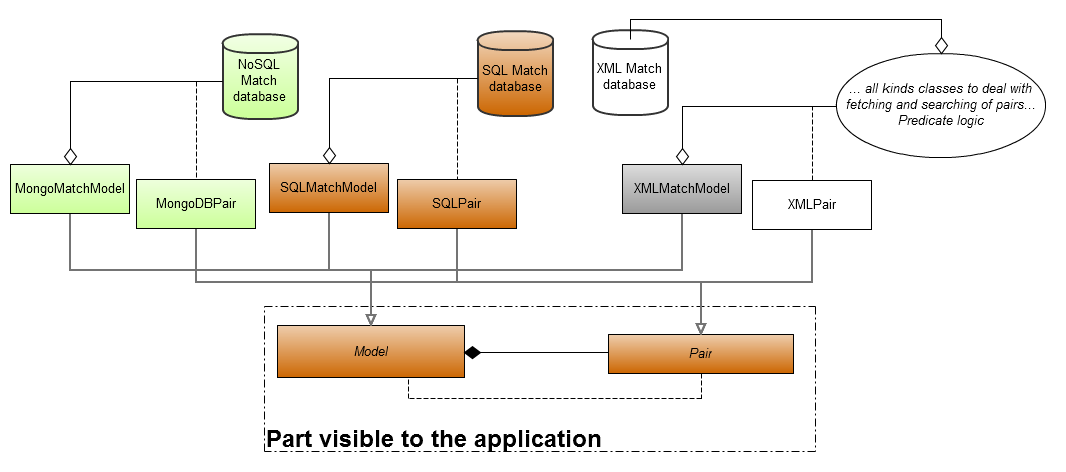
\includegraphics[width=1.0\columnwidth]{images/databaselayer.png}
		\caption{Overzicht van het database systeem, links (groen) is een mogelijke uitbreiding, het middelste deel (oranje) stelt de thesis voor en helemaal rechts (wit) staan de componenten van het thera project.}
		\label{fig:databaselayer}
	\end{center}
\end{figure}

\section{Implementatie}
Ondanks de simpliciteit van de te modelleren data zijn er verscheidene manieren om dit te doen binnen het relationele concept. In figuur~\ref{fig:databasemodel} staat een schematisch model dat moet omgezet worden in SQL tabellen. Het staat buiten twijfel dat tenminste de geschiedenis en de gebruikers in een aparte tabel moeten: voor elk attribuut kunnen er immers verschillende rijen in een geschiedenistabel staan, en meerdere rijen in een geschiedenistabel kunnen door dezelfde gebruiker veroorzaakt zijn. Attributen zouden als kolommen in de ``voorstel'' tabel kunnen gaan, of elk een eigen tabel hebben. De eerste versie komt min of meer overeen met hoe een NoSQL \emph{document} database dit zou voorstellen. Het voordeel van de kolom-aanpak (die \emph{de}normaler is dan de tabel-aanpak) bestaat uit een grotere snelheid bij het opvragen (geen JOINs\footnote{Het commando om twee tabellen met elkaar te verbinden heet een JOIN in SQL. Hoewel de database dit expliciet voorziet en opsplitsen in tabellen aangemoedigd wordt, is het verbinden van veel tabellen vaak nefast voor de performantie.}). Bovendien neemt het minder ruimte in op de harde schijf omdat er geen verwijzingen moeten bijgehouden worden voor elk attribuut. Het laatste voordeel voert de snelheid nog eens op want er kan zo meer data in het werkgeheugen blijven. Anderzijds laat de tabel-aanpak toe om attributen te defini\"eren die niet voor alle fragmentparen bestaan, bijvoorbeeld als slechts 1000 van het miljoen paren een commentaar bevat. Op die manier kan afhankelijk van de verdeling van de attributen zelfs nog meer ruimte bespaard worden. SQLite, de implementatie voor kleine lokale kopie\"en kan ook geen kolommen verwijderen van een tabel. Omdat het eenvoudig is de tabel-aanpak om te zetten in de kolom-aanpak is deze preferibel om te beginnen. De eigenlijk beslissing kan uitgesteld worden tot wanneer blijkt dat er performantieproblemen zijn.\\

\begin{figure}[ht]
	\begin{center}
		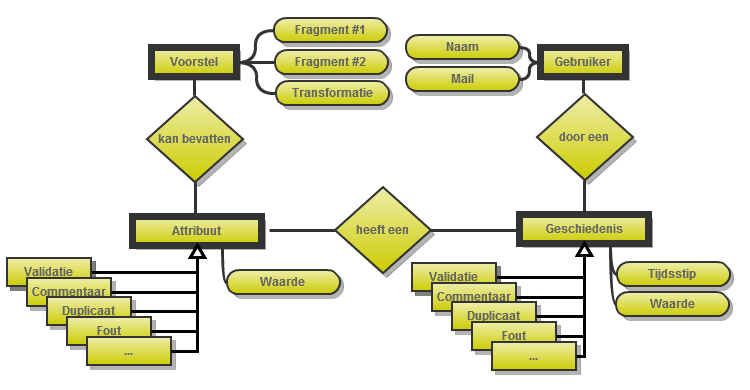
\includegraphics[width=1.0\columnwidth]{images/databasemodel.png}
		\caption{Een relationele modellering van de data}
		\label{fig:databasemodel}
	\end{center}
\end{figure}

\subsection{Normale attributen}
Dit model heeft een groot voordeel: het is voorspelbaar maar uitbreidbaar. De voorspelbaarheid van het attribuut-formaat zorgt ervoor dat queries automatisch kunnen gegenereerd worden, omdat elk veld aan een specifieke structuur voldoet. Steeds is het mogelijk om attributen toe te voegen en te verwijderen: de databaselaag ``herkent'' elke tabel die eruitziet als een attribuut en brengt alle ge\"interesseerde componenten hiervan op de hoogte.

\subsection{Complexe attributen}
De (verplichte) voorspelbaarheid van de attributen kan ook op een dwangbuis lijken: er is zeker informatie denkbaar die niet simpelweg in \'e\'en kolom past of gaat over meer dan \'e\'en paar tegelijkertijd. In extremis is het mogelijk om dit soort data toe te voegen en te onderhouden door een module te schrijven. Er bestaan dan tabellen waarmee de databaselaag niet kan werken, maar de module kan wel via ruwe queries aan die data. Dit heeft natuurlijk het nadeel dat een heel deel van de infrastructuur op die manier ontweken wordt. Andere modules kunnen deze data niet ``ontdekken'' en weergeven en de queries worden niet automatisch geoptimaliseerd. Filters en sorteeroperaties zijn dan ook niet toegankelijk via de normale interface.\\

Een oplossing hiervoor zijn meta-attributen. Deze zijn niet schrijfbaar omdat ze opgemaakt zijn uit samengestelde data van andere tabellen. Voor de rest gedragen ze zich exact zoals normale attributen. Dit wil zeggen dat ze automatisch kunnen ontdekt en gebruikt worden. Het beste hieraan is dat dit allemaal in de declaratieve taal van de database kan gebeuren, waardoor extra modules of een hercompilatie van het programma niet nodig zijn.\\

Deze functionaliteit wordt ge\"implementeerd met behulp van SQL Views, een manier om een verzoek als een tabel voor te stellen. Als er een verzoek op onregelmatig gevormde data kan gemaakt worden dat \textbf{lijkt} op een attribuut, kan dit een meta-attribuut zijn. Om de zojuist beschreven zaken wat minder abstract te maken, volgt een voorbeeld van een twee echte meta-attributen:\\

\subsubsection{Duplicaten}
De automatische herkenners stellen soms paren voor die hard op elkaar gelijken maar niet exact dezelfde zijn (zie figuur~\ref{fig:duplicates}). Om data-analyse redenen worden deze niet automatisch verworpen, ze hebben licht verschillende eigenschappen en het kan nuttig zijn deze te onderzoeken.\\

\begin{figure}[ht]
	\begin{center}
		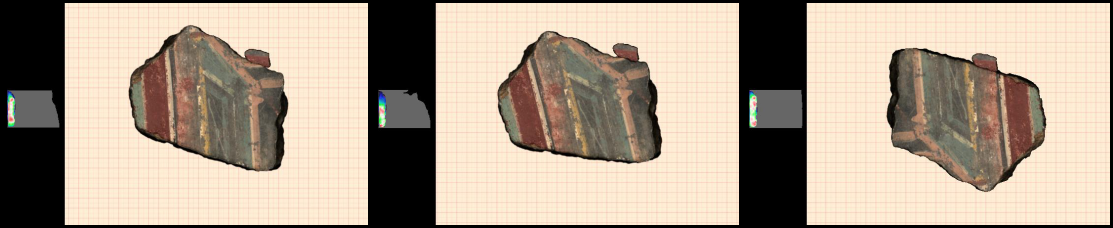
\includegraphics[width=1.0\columnwidth]{images/duplicates.png}
		\caption{Duplicaten: het tweede paar is een duplicaat van het eerste, het derde niet.}
		\label{fig:duplicates}
	\end{center}
\end{figure}

Als men niet specifiek op zoek is naar duplicaten, is het dikwijls beter om enkel het beste paar uit een groep duplicaten te laten zien. Tegelijkertijd moet de gebruikersomgeving een visuele hint kunnen geven dat een bepaald voorstel enkele duplicaten heeft. Opslaan welk paar representatief is, kan nog voorgesteld worden als een attribuut. De waarde van dit attribuut, ``duplicaat'' genaamd, is een verwijzing naar het representatieve paar van de groep of het getal 0. Als de waarde 0 is, geeft dit aan dat een paar de beste uit zijn groep is (elk paar is dus in het begin de beste uit de groep die alleen het paar zelf bevat). Als men wil aanduiden dat een groep paren een duplicaat is van een ander, volstaat het om de waarde van hun ``duplicaat''-attribuut op het identificatienummer van dit paar te zetten.\\

Er is slechts \'e\'en probleem over: door te kijken naar het ``duplicaat''-argument kan men niet weten of dit paar duplicaten heeft of niet (enkel of het een duplicaat of een representatief paar is). Op het eerste zicht lijkt het nodig een apart attribuut ``aantal\_duplicaten'' bij te houden en dit telkens aan te passen als er ergens in ``duplicaat'' een verwijzing verandert. Dit is mogelijk maar zeer gevoelig voor corruptie (desynchronisatie van beide tabellen). Eigenlijk kan het aantal duplicaten rechtstreeks uit het ``duplicaat''-attribuut worden gehaald: voor het paar waarvan men wil weten of het een duplicaat heeft, tel hoeveel ernaar verwijzen. Een apart attribuut bijhouden zou dus redundant zijn. Deze telsom valt in een SQL-verzoek te vertalen:

\lstinputlisting[label=code:duplicates,caption=Deze query kan als view dienen om het aantal duplicaten per paar als meta-attribuut te gebruiken, language=SQL]{source/duplicates.sql}

De databaselaag kan van deze zin een meta-attribuut maken dat aangeeft hoeveel duplicaten een paar heeft. Het gedraagt zich als een extra tabel maar is in feite gewoon een datatransformatie. De \emph{MatchTileView} module die later wordt besproken kiest ervoor om dit meta-attribuut weer te geven door een paar laagjes onder een afbeelding van het paar te tekenen, zoals in figuur~\ref{fig:duplicatesdone}.

\begin{figure}[!h]
	\begin{center}
		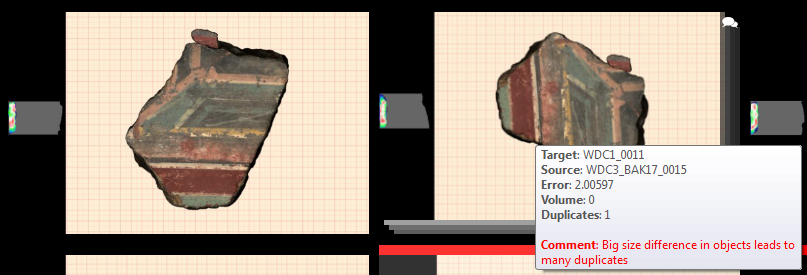
\includegraphics[width=1.0\columnwidth]{images/duplicates-2.png}
		\caption{Duplicaten: het tweede paar van figuur~\ref{fig:duplicates} verwijst nu naar het eerste paar}
		\label{fig:duplicatesdone}
	\end{center}
\end{figure}

\subsubsection{Correspondentie}
Een ander voorbeeld van een meta-attribuut is correspondentie. Alle commentaren die ooit op een fragment zijn gegeven kunnen aan elkaar worden gezet! Een voorbeeld van een query die hiervoor kan dienen is broncode~\ref{code:correspondence}\\

\lstinputlisting[float=htpb,label=code:correspondence,caption=Deze query kan als view dienen om de geschiedenis van een ``commentaar''-attribuut om te vormen tot een ``correspondentie''-attribuut, language=SQL]{source/correspondence.sql}

Zo zijn er nog vele andere meta-attributen denkbaar, er is geen beperking op hoeveel tabellen er moeten gecombineerd worden om het te verkrijgen zolang het resultaat maar de vorm van een normaal attribuut heeft.

\subsection{Querygeneratie}
Omdat verschillende modules en bij extensie gebruikers andere noden hebben, worden de verzoeken naar de database steeds opnieuw gegenereerd uitgaande van een stel parameters.\\

De eerste iteratie van het systeem was zeer eenvoudig: een query bestond uit een sorteerveld, sorteerrichting en een enkele filter op een attribuut. Dit werkte acceptabel voor kleine collecties zoals degene waar Browsematches en Griphos mee moeten werken, maar was niet echt vernieuwend.\\

Een aanzienlijk probleem was bijvoorbeeld dat alle fragmenten die voldeden aan de filtercriteria werden opgehaald. Een duizendtal paren van een SQL implementatie die lokaal draait (of zelfs volledig in het geheugen, zoals SQLite) is snel. Tienduizenden paren gaat niet meer zo vlot. Niet alleen nemen die veel geheugen in, de informatie in het verzoek moet elke keer verwerkt worden en omgezet in evenveel C++ objecten. Dit is vooral traag omwille van de opslag van de transformatiematrix als pure tekst, die telkens omgezet wordt naar een matrix van (32-bit) decimale getallen. De tekstopslag laat arbitraire precisie toe, wat belangrijk is om het voorstel van de automatische herkenner zo getrouw mogelijk te maken. De volgende subsecties bespreken eerst hoe filters mogelijk zijn en daarna enkele optimalisaties die het systeem effici\"ent maken voor grote datasets en over (trage) netwerkverbindingen.

\subsubsection{Filters}
In hoofdstuk~\ref{hoofdstuk:ontwerp} werd reeds uit de doeken gedaan dat er meerdere filters tegelijkertijd mogelijk zijn. Alle attributen zitten opgeslagen in aparte tabellen, in SQL moet een query deze expliciet vermelden. Aangezien de filters willekeurige tekst zijn die hopelijk welgevormde SQL voorstellen, is een tekstanalyse nodig om te bepalen op welke attributen ze steunen. Dit wordt gedaan met reguliere expressies\footnote{Een formele taal die het mogelijk maakt om ingewikkelde patronen in tekst te herkennen.}. Alle filters worden conjunctief (met het ``AND'' sleutelwoord) in een WHERE-clausule gezet en alle ontdekte afhankelijkheden worden met een ``JOIN'' in het domein gebracht.\\

Merk op dat indien eerder de kolom-aanpak --- d.w.z. alle attributen als extra kolommen in de parentabel --- was genomen, deze tekstanalyse niet nodig zou geweest zijn. Gelukkig blijkt de analyse nuttig voor andere optimalisaties die hieronder worden beschreven. 

\subsubsection{Standaardisatie}
Ondanks het feit dat SQL een gestandaardiseerde taal is, gebruikt elke implementatie wel een eigen dialect. Daarom loopt een preprocessor steeds door de volledige query om de dialecten te unificeren, ook hiervoor worden reguliere expressies ten volle benut.

\subsubsection{Paginatie}
Tienduizenden paren ophalen werd al aangegeven als een oorzaak van traagheid, zelfs op lokale installaties. Hetzelfde probleem doet zich nog veel erger voor als de verbinding naar de database over het netwerk loopt. Zonder de effici\"entieverliezen van de databaseopslag neemt elk paar zonder attributen ongeveer 924 bytes in\footnote{Het grooste deel hiervan is afkomstig van de tekstvoorstelling van de transformatiematrix}. Het is niet ongewoon om verzamelingen van 10000 paren te weerhouden, wat een ondergrens van 8.8MB over het netwerk zou betekenen. Een redelijk doel lijkt om alle verzoeken binnen een seconde af te werken, wat niet mogelijk is met zulke hoeveelheden data.\\

Om die reden zal het model bijna nooit de volledige set aan de database opvragen, maar slechts een klein deeltje. Allereerst wordt aan de database gevraagd hoeveel paren aan de criteria voldoen, zodat het model kan rapporteren dat het X aantal paren in bezit heeft. Dit laadt ook meteen veel noodzakelijke data in het werkgeheugen van de server. Als een component dan vraagt om een bepaald paar, zal het model kijken of de aanvraag binnen het bereik van het huidige venster past. Indien niet, wordt het venster opgehaald waarin de aanvraag wel past. Dit proces is transparant voor de componenten die van het model gebruik maken. Ze kunnen de parameters zoals venstergrootte wel be\"invloeden door hints te geven, hoewel het model niet verplicht is deze te volgen. Dit is vooral handig voor componenten die een willekeurig toegangspatroon naar de data hebben, waarvoor vensters bijzonder ineffici\"ent zijn omdat er bij elke aanvraag een volledig nieuw venster opgehaald wordt.

\subsubsection{Voorladen}
Een component kan aan een fragmentpaar vragen welke waarde het heeft voor een bepaald attribuut. De eerste versies van zo'n fragmentpaar-objecten vuurden een query af naar de database elke keer een attribuut opgevraagd werd. Dit is eenvoudig en zorgt ervoor dat de waarde altijd zo actueel mogelijk is. De query op zich is bijzonder eenvoudig en kan razendsnel afgehandeld worden door de database. In een venster van de belangrijkste module passen 20 fragmentparen. De module heeft van elk paar ongeveer 5 attributen nodig om weer te geven, dit geeft 100 extra verzoeken aan de database na het ophalen van de paren zelf. Voor een lokale server is dit geen probleem, maar als de verzoeken over het netwerk moeten komt er tenminste 100 maal de heen-en-weer tijd van een netwerkpakket bij.\footnote{Queries worden niet parallel uitgevoerd}\\

Onafhankelijk van de snelheid van het verzoek maakt deze techiek werken over het netwerk te traag. Om die reden beschikt elk fragmentpaar over een datastructuur waarin het eerst zal kijken of het geen lokale kopie van het attribuut heeft. De querygenerator werd voorzien van de capabiliteit om een parameter ``voorlaadvelden'' aan te nemen, die ervoor zorgt dat een paar reeds voorgevuld wordt met de gevraagde attributen. Het aantal queries per venster loopt dan terug naar 1. Dit heeft geen impact op de versheid van de data, de attributen worden in ieder geval slechts bij het laden van het venster opgevraagd.

\subsubsection{Geforceerde indexen}
Een index is een versnellingsstructuur die de database toelaat om niet de volledige collectie af te gaan bij elk verzoek. Meestal gaat het hier over een binaire boom die ervoor zorgt dat queries op exacte waarden en bereiken (vb. $error < 0.50140$ $\land$ $error > 0.45713$) zeer snel gaan. Indexen zijn gedefinieerd per kolom of groepering van kolommen, het voorbeeld van daarnet heeft dus een index op de ``error'' kolom nodig. Dit is \'e\'en van de zaken die het predicaten-systeem van het thera project mistte.\\

De query planner van MySQL en SQLite is niet zo geavanceerd als die van de commerci\"ele databases, en maakt daarom nogal eens grove fouten als het aankomt op het kiezen van de juiste index. Meer nog, deze twee implementaties zijn gelimiteerd tot \'e\'en index per query, en als deze verkeerd gekozen wordt kan dat soms desastreuze gevolgen hebben voor de snelheid. Om deze cruciale beslissing te maken kijken zij vooral naar de selectiviteit. Samengevat: de query planner kiest over het algemeen de index voor de conditie die de dataset hopelijk het meest verkleint. Als er geen condities maar wel een gesorteerd resultaat is aangevraagd, zal de planner een index gebruiken om te sorteren als die bestaat (binaire bomen worden gesorteerd bijgehouden).\\

Het probleem is dat deze heuristiek geen rekening houdt met een paar belangrijke zaken. Stel een database met een miljoen paren voor en een conditie in een query brengt dit terug naar een half miljoen ongesorteerde paren. Indien er toch gesorteerd moet worden, moet dat in situ gebeuren, zonder een index. Dit is reeds zeer traag op zich. Daarbovenop past zo'n resultaat niet in het werkgeheugen, dus de database sorteert in stukjes door het resultaat weg te schrijven naar het bestandssysteem. Dit gebeurt allemaal ondanks het feit dat er uiteindelijk slechts enkele paren opgevraagd worden.\\

Daarom is het beter om in dit geval selectiviteit te laten voor wat het is en een index te gebruiken om het resultaat reeds gesorteerd op te vragen. Op die manier moet er geen tijdelijk bestand aangemaakt worden. De querygenerator van dit project is geavanceerd genoeg om te detecteren wanneer het beter is om een sorteerindex te forceren en doet dit dan ook.

\subsubsection{Snelle paginatie}
Paginatie is goed om de hoeveelheid getransfereerde data te minimaliseren, maar de simpele vorm is traag voor grote databases gecombineerd met vensters ver in de dataset. Zo kan een query die voor venster $[100, 120]$ nog binnen de 50 milliseconden afgewerkt kan worden, plots 7000 milliseconden duren voor venster $[10000, 10020]$. De reden heeft onder andere te maken met het feit dat voor de tweede query alle 10000 rijen die niet moeten opgehaald worden toch worden nagekeken. De database kan niet op voorhand weten welke rij precies de 10000'ste is onder de geldende criteria. Bij grote databases is het erg waarschijnlijk dat deze 10000 rijen niet in elkaars buurt staan op de harde schijf. Dit verklaart de lange zoektijd.\\

Een oplossing is om de database contextinformatie mee te geven~\cite{sqlfastpag}. Als het vorige opgevraagde venster afdalend gesorteerd was op de \emph{fout}, dan zal het volgende venster beginnen met een \emph{fout} kleiner of gelijk aan de fout van het einde van het huidige venster. Door dit mee te geven in conditie kan de database gebruik maken van een index en zo de opvraagtijd dramatisch inkorten. Voor dit project is deze techniek uitgebreid geweest naar een krachtigere variant die ``relatieve positionering'' werd gedoopt. Dit wil gewoon zeggen dat de querygenerator altijd de meest dichtbijzijnde gekende waarde zal gebruiken om een nieuw venster op te halen.

\subsubsection{Late rijopzoeking}
Late rijopzoeking is uiteindelijk de meest effectieve optimalisatie van allemaal. Het maakt sommige queries zo snel dat het effect van de andere optimalisaties niet meer te merken is. E\'en van de voornaamste redenen waarom queries traag zijn is dat elke keer er een waarde uit een rij nodig is, alle gevraagde kolommen worden opgehaald, niettegenstaande of de rij nu in het uiteindelijke resultaat zit of niet. Als het veld dat nagekeken moet worden een simpel geheel getal is van 4 bytes, is het bijzonder kwistig om meteen nog eens een slordige 1000 bytes aan misschien onnodige informatie op te halen. Om de zaken erger te maken staan deze 1000 bytes met grote kans opnieuw niet dicht bij elkaar op de harde schijf\footnote{Dit proximiteitsargument is niet van toepassing op \emph{Solid State Drives}}, wat voor hoge zoektijden zorgt.\\

Dit slecht gedrag ontwijken kan door middel van een subquery. Het basisidee is: de binnenste query reduceert de dataset zoveel mogelijk en haalt enkel de nodige informatie op om de correcte rijen te identificeren (een sleutel), terwijl de buitenste query al de nodige informatie ophaalt aan de hand van die sleutel. Met een venster kunnen er dus nooit meer rijen volledig opgehaald worden dan de venstergrootte.\\

Om de binnenste query zo effici\"ent mogelijk te maken is het voordelig te weten welke velden en tabellen nodig zijn om de dataset te reduceren en welke kunnen doorgeschoven worden naar de buitenste query. Dat is waar de afhankelijkheidsanalyse van daarstraks goed van pas komt.\\

Normaalgezien zou de queryplanner van de database deze optimalisatie zelf moeten uitvoeren, maar zowel SQLite, MySQL en verassend genoeg PostgreSQL\footnote{De queryplanner van PostgreSQL staat bekend als een van de meest geavanceerde, en zou zelfs specifiek late rijopzoeking ondersteunen.} leken hier (veel) voordeel bij te halen.

\subsubsection{Experimenteel: materialized views}
Een spijtig nadeel van de kracht van meta-attributen is dat ze queries sterk vertragen. Hun dynamische aard zorgt ervoor dat de achterliggende query steeds wordt uitgevoerd voor elk verzoek. Een rij ophalen van ``aantal\_duplicaten'' impliceert op die manier een volledige scan de ``duplicaat'' tabel. Vele oplossingen voor dit probleem werden getest maar geen enkele bracht de nodige verbetering of waren slechts van toepassing op een beperkte subset van de mogelijke verzoeken. Het enige wat overbleef was doen wat meta-attributen net proberen te vermijden: een echte tabel maken van de view. Natuurlijk moest dit gebeuren zonder de nadelen van een echte tabel die niet gedesynchroniseerd kan geraken met de originele tabellen.\\

Het concept op zich heet een gematerialiseerde view. De opzet is om een automatische verbinding te maken tussen de moedertabellen en het meta-attribuut, zodat elke update gepropageerd wordt. Dit is een simpel uitgangspunt, maar heeft een verassend moeilijke uitwerking. De huidige implementatie is zeer rudimentair en werkt alleen in PostgreSQL, de implementatie met de meest geavanceerde programmeermogelijkheden. De resultaten zijn echter veelbelovend, zie sectie~\ref{sec:benchmarks}.

\subsection{Collaboratie}
De verschillende optimalisaties uit de vorige secties maken het mogelijk om een externe database te gebruiken en toch met grote snelheid te navigeren in de dataset. Dit betekent dat iedereen steeds de meest actuele data te zien krijgt. In deze opstelling is synchronisatie niet nodig, zolang er een netwerk- of internetverbinding beschikbaar is. Als meerdere gebruikers tegelijkertijd met dezelfde paren aan het werken zijn, zullen ze elkaars veranderingen niet zien verschijnen tot ze het venster vernieuwen. Voor deze situatie is een oplossing gemaakt die gebruikmaakt van het feit dat de meeste queries snel afgehandeld worden. Als het model merkt dat het ophalen van een venster snel gaat, zal het periodisch proberen dit venster te vernieuwen. De periode past zich aan de omstandigheden aan, hoe langer het duurt om een venster op te vragen, hoe langer het model zal wachten. Dit is zo omdat de reden voor de traagheid misschien een overbelasting van de database is.\footnote{Ge\"inspireerd door het dynamisch gedrag van het TCP pakketprotocol}\\

Dankzij dit systeem verschijnen de laatste nieuwe veranderingen steeds op het scherm van de gebruiker, zodat geen dubbel werk wordt verricht.

\section{Data mining}
Maak ketting van (yes+maybe) ---> zoek naar alle buren binnen 1 hop (algoritme is geschreven) --- FINDNEIGHBOURS.SQL

Meer mogelijkheden: geef alle paren die recent zijn aangepast.


\section{Benchmarks}
\label{sec:benchmarks}
Er zijn reeds een paar namen gevallen van gebruikte database implementaties: SQLite, MySQL en PostgreSQL. In het begin draaide 
Dankzij de flexibiliteit die nodig was om zowel SQLite als MySQL het grootst mogelijke deel van de code te laten delen

\subsection{Indexering}
Analyse van datatoegangspatroon: vooral SELECT, ORDER BY, GROUP BY ---->
veelvuldig gebruik van indexes

optimize voor fast reads -----> inserts kunnen lokaal gedaan worden, updates hopelijk niet zo veel of lokaal


\subsection{Opstelling}
Beide databases kregen 512 MB RAM aan werkgeheugen toe. Het is natuurlijk niet mogelijk om exact dezelfde configuratie te krijgen omdat de opties verschillen.

De query cache staat af
Om de variabiliteit van de filesystem (nederlands) cache een beetje buiten spel te zetten zijn al deze routines ``opgewarmd''

Pagination
Late row lookup

Ideaal = minder dan een seconden voor elke gegeven query vanuit een gebruikersinteractie standpunt (System Response Time and User Satisfaction pagina 5)

Effect van DB configuratie (veel geheugen\ldots)

Suggested workaround voor het text probleem -> sphinx, restrict fragment names (niet ZO gemakkelijk), string + nummer
Suggested workaround voor het indexing probleem (zoals gezien voor status IN (\ldots)) -> force een index?! dunno\ldots hij pakt in ieder geval de verkeerde!

'High Performance MySQL', Second Edition, O'REILLY, ISBN: 978-0-596-10171-8
MySQL Reference Manual for version 5.1

http://nlp.stanford.edu/IR-book/html/htmledition/permuterm-indexes-1.html (dit is hoe wildspeed werkt) (LIKE performance lijkt niet zo slecht in Postgres, het is de sorting eerder\ldots)
http://www.slideshare.net/techdude/how-to-kill-mysql-performance
http://stackoverflow.com/questions/1540590/how-to-speed-up-like-operation-in-sql-postgres-preferably <--- use trigrams (fail), MAAR BETER IN 9.1 (future research)
https://cgsrv1.arrc.csiro.au/blog/2010/06/23/materializedindexed-views-for-postgresql/